\documentclass{../../../oss-apphys-exam}
\newcounter{lastmc}
\ctikzset{
  voltage=american,
  misc/scale=.75,
  %bipoles/length=1cm,
  %misc/thickness=.5,
}
\tikzstyle{every node}=[scale=.85]

\begin{document}

\gentitle{11}{CIRCUIT ANALYSIS, PART 1}

\raggedcolumns

\runningheader{
  \fontfamily{phv}\small
  \textcolor{gray}{AP PHYSICS C: ELECTRICITY AND MAGNETISM $\blacksquare$}
  \textbf{MULTIPLE-CHOICE QUESTIONS}}{}{}


\begin{questions}
  \question Five resistors are made of the same material. Which of the
  following has the highest resistance?

  \begin{oneparchoices}
    \choice
    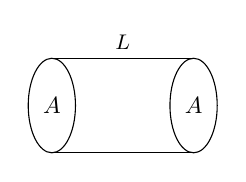
\begin{tikzpicture}[scale=.6]
      \draw ellipse (.5 and 1) node{$A$};
      \draw (3,0) ellipse (.5 and 1) node{$A$};
      \draw (0,1)--(3,1) node[midway,above]{\small$L$};
      \draw (0,-1)--(3,-1);
    \end{tikzpicture}
    \choice
    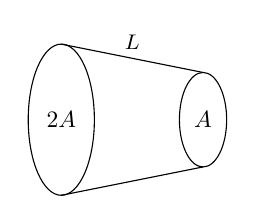
\begin{tikzpicture}[scale=.6]
      \draw ellipse (.7 and 1.6) node{$2A$};
      \draw (3,0) ellipse (.5 and 1) node{$A$};
      \draw (0,1.6)--(3,1) node[midway,above]{\small$L$};
      \draw(0,-1.6)--(3,-1);
    \end{tikzpicture}   
    \choice
    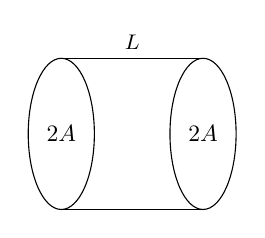
\begin{tikzpicture}[scale=.6]
      \draw ellipse (.7 and 1.6) node{$2A$};
      \draw (3,0) ellipse (.7 and 1.6) node{$2A$};
      \draw (0,1.6)--(3,1.6) node[midway,above]{\small$L$};
      \draw (0,-1.6)--(3,-1.6);
    \end{tikzpicture}
    \choice
    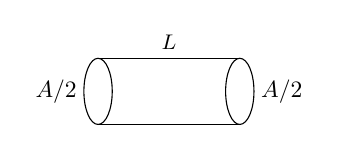
\begin{tikzpicture}[scale=.6]
      \draw ellipse (.3 and .7) node[left]{$A/2\;\;$};
      \draw (3,0) ellipse (.3 and .7) node[right]{$\;\;A/2$};
      \draw (0,.7)--(3,.7) node[midway,above]{\small$L$};
      \draw (0,-.7)--(3,-.7);
    \end{tikzpicture}\\
    \choice
    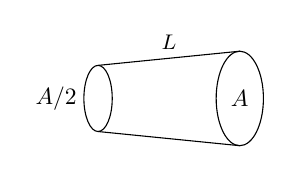
\begin{tikzpicture}[scale=.6]
      \draw ellipse (.3 and .7) node[left]{$A/2\;\;$};
      \draw (3,0) ellipse (.5 and 1) node{$A$};
      \draw (0,.7)--(3,1) node[midway,above]{\small$L$};
      \draw (0,-.7)--(3,-1);
    \end{tikzpicture}
  \end{oneparchoices}
    
  \uplevel{
    \centering
    \begin{tikzpicture}[thick,scale=2.5]
      \draw (0,0) to[battery,l=$\mathcal E$] (0,1)--(1,1)
      to[R,l=$R_1$] (1,.5) to[R,l=$R_2$] (1,0)--(0,0);
      \draw (1,1)--(1.5,1) to[R,l=$R_3$] (1.5,0)--(1,0);
      \draw[fill=white] (.8,0) circle (.1) node{A};
      \draw (.5,1)--(.5,0);
      \draw[fill=white] (.5,.5) circle (.1) node{V};
    \end{tikzpicture}
  }
  \question In the circuit shown, what effect would removing resistor labelled
  $R_2$ have?
  \begin{choices}
    \choice The reading on the voltmeter would increase.
    \choice The reading on the ammeter would increase.
    \choice The reading on the voltmeter would decrease.
    \choice The reading on the ammeter would decrease.
    \choice The reading on the ammeter would not change.
  \end{choices}
    
  \question The current flowing in a wire as a function of time is given by
  the equation $I=4t^3$. The charge that passes through the wire from
  \SI0{\second} to \SI2{\second} is
  \begin{choices}
    \choice\SI2\coulomb
    \choice\SI4\coulomb
    \choice\SI8\coulomb
    \choice\SI{16}\coulomb
    \choice\SI{24}\coulomb
  \end{choices}
  
%    \question Which of the following statements best summarizes a series circuit
%    with three different resistances?
%    \begin{choices}
%      \choice In all parts of the circuit, the resistances are different, the
%      voltage drops are the same, and the current is different.
%      \choice In all parts of the circuit, the resistances are the same, the
%      voltage drops are the same, and the current is different.
%      \choice In all parts of the circuit, the resistances are different, the
%      voltage drops are different, and the current is the same.
%      \choice In all parts of the circuit, the resistances are different, the
%      voltage drops are the same, and the current is the same.
%      \choice In all parts of the circuit, the resistances are the same, the
%      voltage drops are the same, and the current is the same.
%    \end{choices}
%    \uplevel{
%      \cpic{.35}{3batteries}
%%      \centering
%%      \begin{tikzpicture}[yscale=1.5,xscale=1.2]
%%        \draw(5,2)--(5,1) to[R,*-](3,1) to[battery,-*](0,1)--(0,2);
%%        \draw(5,1)--(5,0)--(3,0) to[battery](0,0)--(0,1);
%%        \draw(5,2)--(3,2) to[battery=\mbox{\SI6\volt}](0,2);
%%      \end{tikzpicture}
%    }
%    \question There are three batteries in the circuit shown above. There may
%    be other resistances not shown on the diagram. The potential difference
%    between points $a$ and $b$ is
%    \begin{choices}
%      \choice\SI{3}\volt
%      \choice\SI{6}\volt
%      \choice\SI{9}\volt
%      \choice\SI{12}\volt
%      \choice\SI{18}\volt
%    \end{choices}
  \newpage
  
  \uplevel{
    \textbf{Questions \ref{adjust1}--\ref{adjust2}} A variable resistor is
    connected to a battery of emf $\mathcal E$ in a simple circuit. A graph of
    power vs.\ current in the battery is shown in the figure.
    \cpic{.45}{adjustable}
  }
  \question The emf $\mathcal E$ of the battery is most nearly
  \label{adjust1}
  \begin{choices}
    \choice 5 V
    \choice 10 V
    \choice 20 V
    \choice 40 V
    \choice 60 V
  \end{choices}
    
  \question What is the resistance of the variable resistor when the power
  in the circuit is 10 watts?
  \label{adjust2}
  \begin{choices}
    \choice\SI{1.25}\ohm
    \choice\SI{1.5}\ohm
    \choice\SI{2.5}\ohm
    \choice\SI{5.0}\ohm
    \choice\SI{0}\ohm
  \end{choices}    
    
  \uplevel{
    \textbf{Questions \ref{series1}--\ref{series2}}
    \cpic{.45}{r-in-series}
  }

  \question Which is the correct ranking of the currents for the resistors?
  \label{series1}
  \begin{choices}
    \choice$I_A=I_B=I_C$
    \choice$I_A>I_B>I_C$
    \choice$I_C>I_A=I_B$
    \choice$I_C>I_B>I_A$
    \choice$I_C<I_B<I_A$
  \end{choices}

  \question Which is the correct ranking of the potential differences of the
  resistors?
  \label{series2}
  \begin{choices}
    \choice $V_A=V_B=V_C$
    \choice $V_A>V_B>V_C$
    \choice $V_A=V_B>V_C$
    \choice $V_C>V_B>V_A$
    \choice $V_C<V_B<V_A$
  \end{choices}    
    
  \uplevel{
    \textbf{Questions \ref{bulb1}--\ref{bulb2}}: Four identical light bulbs
    are connected to a battery as shown.
    \cpic{.35}{bulbs}
  }
  \question Which bulb will burn the brightest?
  \label{bulb1}
  \begin{choices}
    \choice 1
    \choice 2
    \choice 3
    \choice 4
    \choice All will emit the same brightness.
  \end{choices}
    
  \question If bulb 4 is removed, how will the brightness of each of the bulbs
  change, if at all?
  \label{bulb2}
  \begin{choices}
    \choice Bulb 2 will be less bright.
    \choice Bulb 2 will be brighter.
    \choice Bulb 3 will not change its brightness.
    \choice Bulb 1 will not give off light.
    \choice None of the bulbs will change their brightness.
  \end{choices}

  \uplevel{
    \centering
    \begin{tikzpicture}[scale=1.5]
      \draw[thick] (0,0) to[battery1,l_=$\mathcal E$] (-.6,0)--(-1,0)--(-1,-1)
      to[R,l=$R$] (1,-1)--(1,0)--(.6,0) to[R,l_=$r$] (0,0);
      \draw[dashed,thick] (-.6,-.3) rectangle (.7,.6);
      \draw[axes] (1,-1)--(1,-.5) node[right]{$I$};
    \end{tikzpicture}
    \hspace{.4in}
    \begin{tikzpicture}[scale=1.5]
      \draw[thick] (0,0) to[battery1,l_=$\mathcal E$] (-.6,0)--(-1,0)--(-1,-1)
      to[R,l=$3R$] (1,-1)--(1,0)--(.6,0) to[R,l_=$r$] (0,0);
      \draw[dashed,thick] (-.6,-.3) rectangle (.7,.6);
      \draw[axes] (1,-1)--(1,-.5) node[right]{$I/2$};
    \end{tikzpicture}
  }
  \question When a battery is connected to an external resistance $R$, as shown
  above on the left, there is a current $I$ in the circuit. When the external
  resistance is changed to $3R$, the current changes to $I/2$, as shown above
  on the right. What is the internal resistance $r$ of the battery?
  \begin{choices}
    \choice$R/4$
    \choice$R/2$
    \choice$R$
    \choice$2R$
    \choice$4R$
  \end{choices}
  \newpage
  
  \uplevel{
    \centering
    \pic{.5}{some-resistors}
  }
  \question A circuit contains three identical light bulbs and a switch S
  connected to an ideal battery of \emph{emf} $\mathcal E$, as shown in the
  figure above. The switch is initially open and bulbs A and B have equal
  brightness, while C is not lit. What happens to the brightness of bulbs A and
  B when the switch S is closed and bulb C lights up?
  
  \begin{tabular}{rll}
    & \underline{\textbf{Bulb A}} & \underline{\textbf{Bulb B}}\\
    (A) & Remains the same & Becomes dimmer\\
    (B) & Becomes dimmer   & Becomes dimmer\\
    (C) & Becomes brighter & Becomes dimmer\\
    (D) & Becomes brighter & Not lit\\
    (E) & Remains the same   & Not lit
  \end{tabular}
\end{questions}
\setcounter{lastmc}{\value{question}}
\newpage
  
\runningheader{
  \fontfamily{phv}\small
  \textcolor{gray}{AP PHYSICS C: ELECTRICITY AND MAGNETISM $\blacksquare$}
  \textbf{FREE-RESPONSE QUESTIONS}}{}{}

  
  %TAKEN FROM 2015 AP PHYSICS EXAM FREE-RESPONSE QUESTION E&M.2.
\begin{center}
  \begin{tikzpicture}[scale=1.1]
    \draw[thick] (4,0)--(3,0) to[battery1,l=$\mathcal{E}$] (2,0)
    to[resistor,l=$r$] (1,0)--(0,0)--(0,2) to[vR,l_=$R$] (4,2)
    --(4,0);
    \draw[dashed] (.9,.5) rectangle (2.7,-.9);
    \draw[thick] (.75,2)--(.75,2.75)--(3.25,2.75)--(3.25,2);
    \draw[thick,fill=white] (2,2.75) circle (.25) node{V};
  \end{tikzpicture}
\end{center}

\begin{questions}
  \setcounter{question}{\value{lastmc}}
  \question A student performs an experiment to determine the emf $\mathcal E$
  and internal resistance $r$ of a given battery. The student connects the
  battery in series to a variable resistance $R$, with a voltmeter across the
  variable resistor, as shown in the figure above, and measures the voltmeter
  reading $V$ as a function of the resistance $R$. The data are
  shown in the table below.
  \begin{center}
    \begin{tabular}{|c|c|c|c|c|}
      \hline
      Trial \# & Resistance [\si\ohm] & Voltage [\si\volt] &
      $1/R$ [\si{\per\ohm}] & $1/V$ [\si{\per\volt}] \\
      \hline
      1 & 0.50 & 5.6 & 2.00 & 0.179 \\ \hline
      2 & 1.0 &  7.4 & 1.00 & 0.135 \\ \hline
      3 & 2.0 &  9.4 & 0.50 & 0.106 \\ \hline
      4 & 3.0 & 10.6 & 0.33 & 0.094 \\ \hline
      5 & 5.0 & 10.9 & 0.20 & 0.092 \\ \hline
      6 & 10 &  11.4 & 0.10 & 0.088 \\ \hline
    \end{tabular}
  \end{center}
  \begin{parts}
    \part\textbf{Derive} an expression for the measured voltage $V$. Express
    your answer in terms of $R$, $\mathcal E$, $r$, and physical constants, as
    appropriate.
    \vspace{\stretch1}
    
    \part\textbf{Rewrite} your expression from part \textbf{A} to express
    $1/V$ as a function of $1/R$.
    \vspace{\stretch2}
    \newpage
    
    \part On the grid below, \textbf{plot} data points for the graph of $1/V$
    as a function of $1/R$. Clearly \textbf{scale} and \textbf{label} all axes,
    including units as appropriate.
    \begin{center}
      \vspace{.1in}
      
\begin{tikzpicture}[scale=1.6]
        \draw[gray,step=.2] grid (5,5);
        \draw[thick] grid (5,5);
      \end{tikzpicture}
    \end{center}
    \part \textbf{Draw} a straight line on the above graph that best represents
    the data.
    
    \part Use the straight line from part \textbf{C} to \textbf{calculate}
    values for the following:
    \begin{subparts}
      \subpart $\mathcal E$
      \subpart $r$
    \end{subparts}
    \vspace{\stretch1}
    
    \part Using the results of the experiment, \textbf{calculate} the maximum
    current that the battery can provide.
    \vspace{\stretch1}
    \newpage
    
    \part A voltmeter is to be used to determine the emf of the battery after
    removing the battery from the circuit. Two voltmeters are available to take
    this measurement---one with low internal resistance and one with high
    internal resistance. \textbf{Indicate} which voltmeter will provide the most
    accurate measurement.
    
    \vspace{.05in}
    \underline{\hspace{.4in}} The voltmeter with low resistance will provide
    the most accurate measurement.

    \vspace{.05in}
    \underline{\hspace{.4in}} The voltmeter with high resistance will provide
    the most accurate measurement.

    \vspace{.05in}
    \underline{\hspace{.4in}} The two voltmeters will provide equal accuracy.

    \vspace{.1in}\textbf{Justify} your answer.
  \end{parts}
  \newpage

  %TAKEN FROM 2016 AP PHYSICS EXAM FREE-RESPONSE QUESTION E&M.2.
  \uplevel{
    \centering
    \begin{tikzpicture}[scale=1.5]
      \draw[thick] (0,0) to[battery,l=$\mathcal E$] (0,2)
      to[resistor,l_=$R$] (2,2)
      to[resistor,l=$r$] (2,0)-- (0,0);
      \draw[thick,fill=white] (1,0) circle (.23) node{A};
      \draw[thick] (.4,2)--(.4,2.6)--(1.6,2.6)--(1.6,2);
      \draw[thick,fill=white] (1,2.6) circle (.23) node{V};
    \end{tikzpicture}
  }
  \question The circuit shown above consists of a source of variable \emph{emf}
  $\mathcal E$, an ideal ammeter A, an ideal voltmeter V, a resistor of
  resistance $R$, and a sample of wire with resistance $r$.
  \begin{parts}
    \part How does the current through the wire sample compare with the current
    through the resistor $R$?
    
    \vspace{.05in}
    \underline{\hspace{.3in}} It is greater through $R$.
    
    \vspace{.05in}
    \underline{\hspace{.3in}} It is greater through the sample.
    
    \vspace{.05in}
    \underline{\hspace{.3in}} It is the same through both.
    
    \vspace{.05in}
    \underline{\hspace{.3in}} It depends on the resistance of the sample.

    \vspace{.1in}\textbf{Justify} your answer.
    \vspace{\stretch1}
    
    \part How does the potential difference across the wire sample compare with
    the potential difference across the resistor $R$?
    
    \vspace{.05in}    
    \underline{\hspace{.4in}}It is greater across $R$.
        
    \vspace{.05in}
    \underline{\hspace{.4in}}It is greater across the sample.
        
    \vspace{.05in}
    \underline{\hspace{.4in}}It is the same across both.
        
    \vspace{.05in}
    \underline{\hspace{.4in}}It depends on the resistance of the sample.

    \vspace{.1in}\textbf{Justify} your answer.
    \vspace{\stretch1}
    \newpage
    
    \uplevel{With the sample of wire in place, the emf of the source is set to
      a given value. The current through and potential difference across the
      resistor $R$ are measured. This is repeated for several values of emf,
      and the data are recorded in the table below.
      
      \begin{center}
        \vspace{.1in}
        \def\arraystretch{2}
        \begin{tabular}{|c|c|c|p{.8in}|p{.8in}|}
          \hline
          $\mathcal E$ [\si\volt] & $V_R$ [\si\volt] & $I_R$ [\si\ampere] & &\\
          \hline
          0.250 & 0.179 & 0.162 & & \\ \hline
          0.500 & 0.335 & 0.327 & & \\ \hline
          0.750 & 0.520 & 0.490 & & \\ \hline
          1.000 & 0.670 & 0.687 & & \\ \hline
        \end{tabular}
        \def\arraystretch{1}
      \end{center}
    }

    \part \textbf{Indicate} below which quantities should be graphed to yield a
    straight line that could be used to calculate a numerical value for the
    resistance of the wire sample.
    \label{part2c}

    \vspace{.05in}
    Horizontal axis: \underline{\hspace{.5in}}

    \vspace{.05in}
    Vertical axis: \underline{\hspace{.5in}}

    You may use the remaining columns in the table above, as needed, to record
    any quantities that you indicated that are not given.
  
    \part On the grid below, \textbf{plot} the straight line data points from
    the above table. Clearly \textbf{scale} and \textbf{label} all axes,
    including units if appropriate.
    \uplevel{
      \centering
      \vspace{.1in}
      
\begin{tikzpicture}[scale=1.6]
        \draw[gray,step=.2] grid (5,5);
        \draw[thick] grid (5,5);
      \end{tikzpicture}
      \vspace{.3in}
    }
    \part\textbf{Draw} a straight line that best represents the data.
    
    \part Use your straight line to \textbf{calculate} the value of the
    resistance of the wire sample.
    \vspace{\stretch1}
    \newpage
    
    \part The wire sample has a length of \SI{3.00}{\metre} and a radius of
    \SI{1.00e-3}\metre. \textbf{Calculate} the resistivity of the material from
    which the wire sample is made.
    \vspace{\stretch1}
    
    \part Suppose the ammeter used to collect these data was not ideal.
    \textbf{Indicate} whether the actual value of the resistance of the wire
    sample be greater than, less than, or equal to that calculated in
    part \textbf{F}?

    \vspace{.2in}
    \underline{\hspace{.3in}} Greater than\hspace{.5in}
    \underline{\hspace{.3in}} Less than\hspace{.5in}
    \underline{\hspace{.3in}} Equal to
      
    \vspace{.1in}\textbf{Justify} your answer.
    \vspace{\stretch1}
      
    \part If the ideal voltmeter is replaced by a voltmeter that is not
    ideal and the experiment is repeated, would the readings of the ideal
    ammeter be greater than, less than, or equal to those in the data chart
    before part \textbf{C}?
    
    \vspace{.2in}
    \underline{\hspace{.3in}} Greater than\hspace{.5in}
    \underline{\hspace{.3in}} Less than\hspace{.5in}
    \underline{\hspace{.3in}} Equal to

    \vspace{.1in}\textbf{Justify} your answer.
    \vspace{\stretch1}
  \end{parts}
\end{questions}
\end{document}
